\chapter{Конструкторский раздел}
\label{cha:design}

В данном разделе будут представлены схемы алгоритмов, выбранных для решения задачи, и диаграмма классов.

\section{Алгоритм срединных смещений}

Схема алгоритма срединных смещений изображена на рисунке \ref{fig:brown_mov_alg}.

\begin{figure}[ph!]
	\center{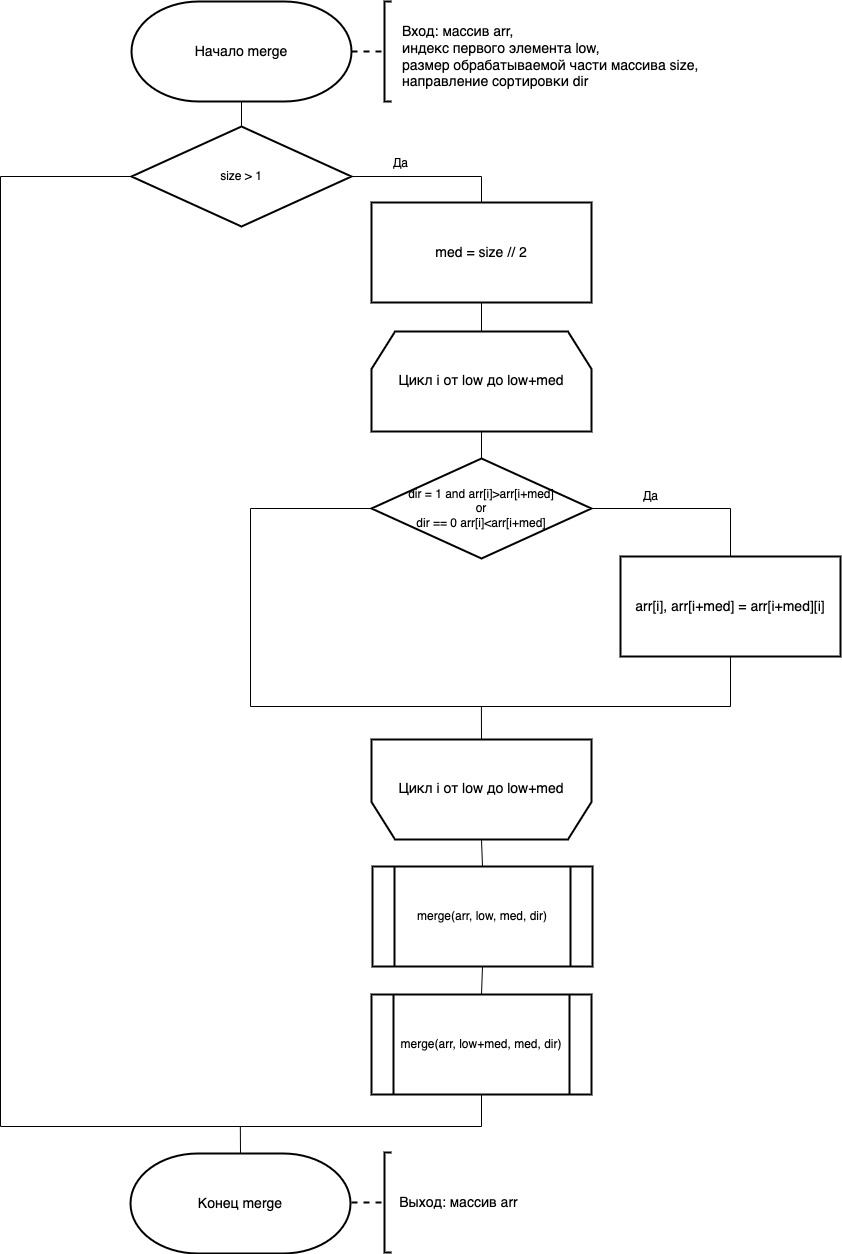
\includegraphics[scale=0.55]{img/bitonic3.png}}
	\caption{Схема алгоритма срединных смещений}
	\label{fig:brown_mov_alg}
\end{figure}

\clearpage

\section{Алгоритмы отрисовки}

Схема алгоритма Z-буфера изображена на рисунке \ref{fig:z_buf_alg}.

\begin{figure}[ph!]
	\center{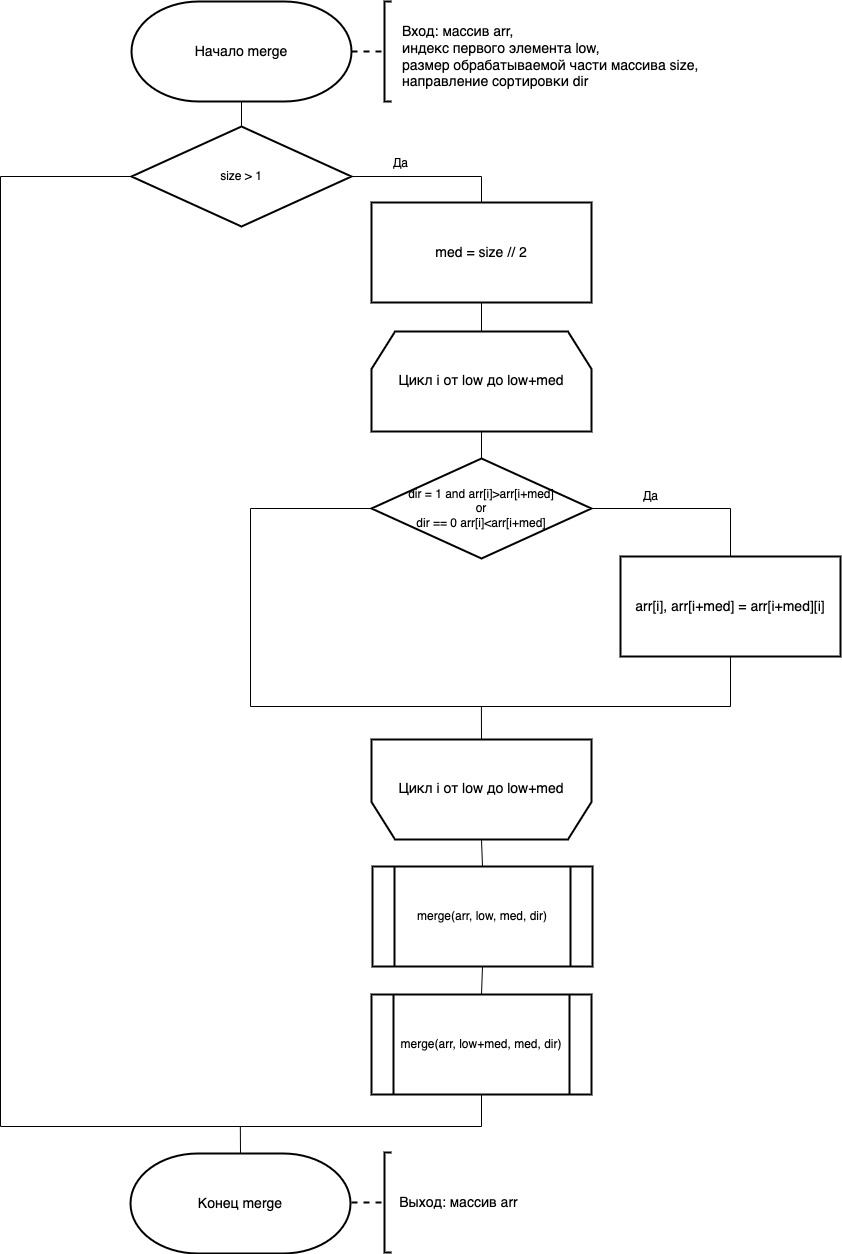
\includegraphics[scale=0.5]{img/bitonic3.png}}
	\caption{Схема алгоритма Z-буфер}
	\label{fig:z_buf_alg}
\end{figure}

\clearpage

Схема алгоритма закраски по Гуро изображена на рисунке \ref{fig:guro_alg}.

\begin{figure}[ph!]
	\center{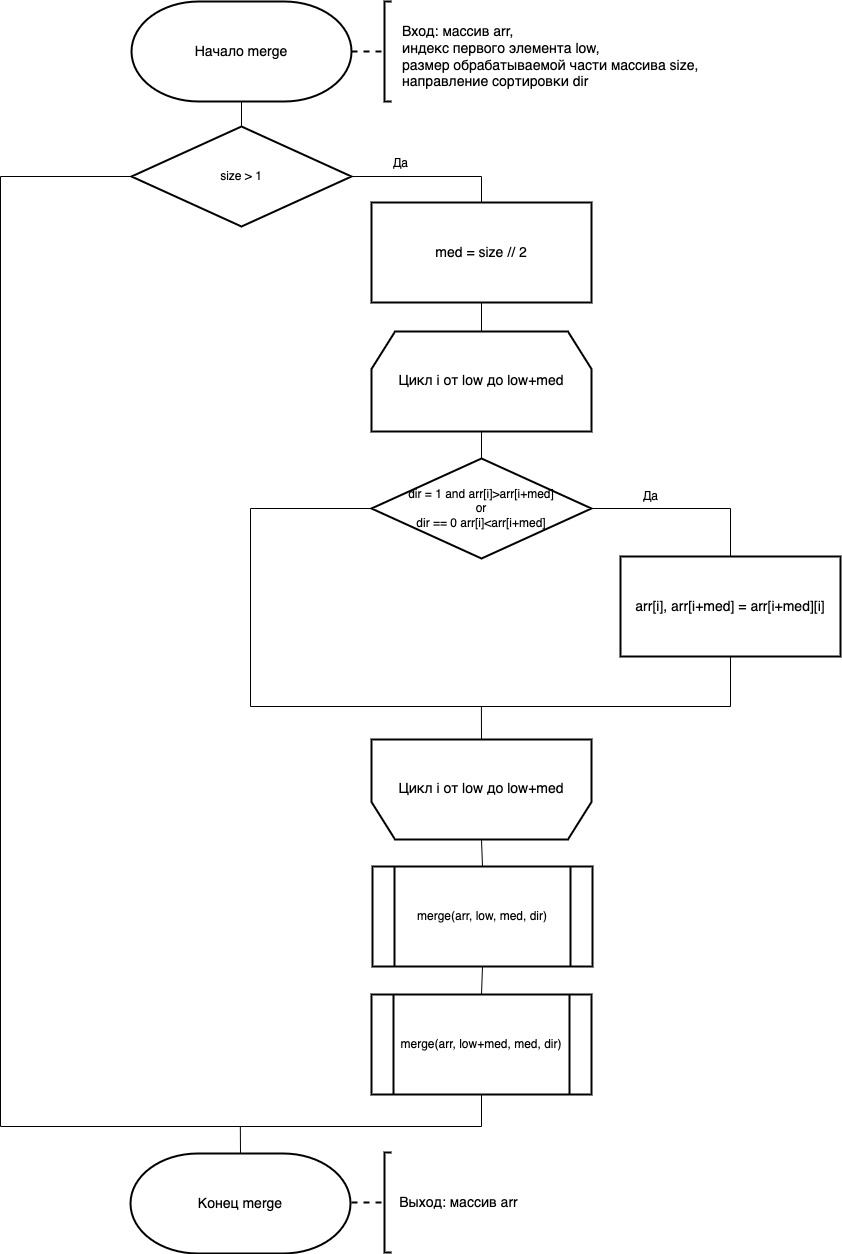
\includegraphics[scale=0.5]{img/bitonic3.png}}
	\caption{Схема алгоритма закраски по Гур}
	\label{fig:guro_alg}
\end{figure}

\clearpage

\section{Диаграмма классов}

На рисунке \ref{fig:diag_class} представлена диаграмма классов.

\begin{figure}[ph!]
	\center{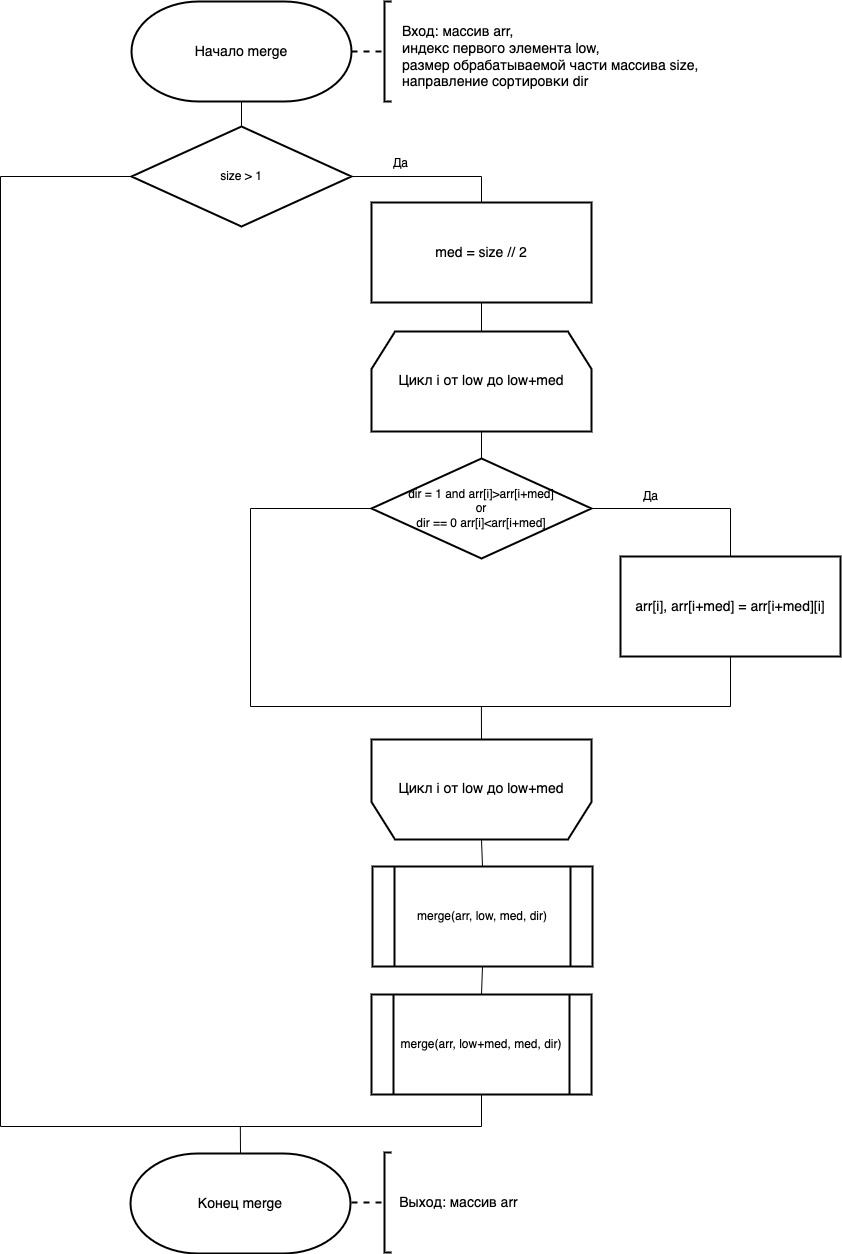
\includegraphics[scale=0.15]{img/bitonic3.png}}
	\caption{Диаграмма классов}
	\label{fig:diag_class}
\end{figure}

Классы объектов сцены:
\begin{itemize}
	\item Model (класс трёхмерных объектов с возможностью перемещения, масштабирования и поворота вокруг собственного центра);
	\item Camera (класс камеры с возможностью перемещения);
	\item LightSourcePoint (класс источника освещения с возможностью)
	перемещения по сцене и изменения мощности.
\end{itemize}

Вспомогательные классы сцены:
\begin{itemize}
	\item  Scene (контейнер, который содержит в себе объекты сцены).
\end{itemize}

\section*{Вывод}
В данном разделе были рассмотрены схемы алгоритмов, использованных при отрисовке сцены, а также диаграмма классов.


